\chapter{Tabelle Hash}

\section{Introduzione}

Le tabelle hash sono tra le strutture dati più utilizzate in informatica pratica. Offrono tempi di ricerca, inserimento e cancellazione \textbf{medi} $O(1)$, prestazioni inarrivabili da altre strutture dati per operazioni di dizionario.

Un dizionario (o mappa) è una collezione di coppie (chiave, valore) che supporta le operazioni:
\begin{itemize}
    \item \texttt{insert(chiave, valore)}: Inserisce una coppia
    \item \texttt{search(chiave)}: Cerca e restituisce il valore associato
    \item \texttt{delete(chiave)}: Rimuove la coppia
\end{itemize}

Le tabelle hash implementano efficientemente queste operazioni tramite una \textbf{funzione hash} che mappa strategicamente le chiavi in posizioni di un array.

\section{Concetti fondamentali}

\begin{definizione}[Funzione hash]
Una \textbf{funzione hash} è una funzione $h: U \to \{0, 1, \ldots, m-1\}$ che trasforma elementi di un universo $U$ (potenzialmente enorme e non limitato) in un insieme ristretto di dimensione $m$ di posizioni all'interno di un array chiamato \textbf{tabella hash}. Questa mappatura comprime l'enorme spazio delle possibili chiavi in un numero gestibile di slot, permettendo un accesso rapido ai dati.
\end{definizione}

\begin{definizione}[Collisione]
Una \textbf{collisione} si verifica quando due chiavi diverse $k_1 \neq k_2$ hanno lo stesso valore hash: $h(k_1) = h(k_2)$.
\end{definizione}

\textbf{Visualizzazione:}

\begin{center}
\begin{tikzpicture}[
    box/.style={rectangle, draw, minimum width=1.2cm, minimum height=0.7cm},
    >=stealth
]
% Universo chiavi
\node at (-3, 3) {Chiavi (U):};
\node[draw, ellipse, minimum width=2cm, minimum height=3cm] at (-3, 1) {};
\node at (-3, 2) {k1};
\node at (-3, 1.2) {k2};
\node at (-3, 0.4) {k3};
\node at (-3, -0.2) {...};

% Funzione hash
\draw[->, thick] (-2, 1.5) -- (0, 1.5) node[midway, above] {$h$};

% Tabella hash
\node at (2, 3) {Tabella hash (T):};
\foreach \i in {0,...,7} {
    \node[box] (t\i) at (2, 2.5-\i*0.4) {};
    \node[left] at (1.3, 2.5-\i*0.4) {\i};
}

% Mapping
\draw[->, red] (-2.3, 2) to[bend left] (t2);
\draw[->, blue] (-2.3, 1.2) to[bend left] (t5);
\draw[->, green!50!black] (-2.3, 0.4) to[bend left] (t2);

\node[right, red] at (3, 2.5-2*0.4) {$h(k1) = 2$};
\node[right, blue] at (3, 2.5-5*0.4) {$h(k2) = 5$};
\node[right, green!50!black] at (3.5, 2.5-2*0.4+0.3) {$h(k3) = 2$ (collisione!)};
\end{tikzpicture}
\end{center}

\textbf{Problema delle collisioni:} Dato che tipicamente $|U| \gg m$, per il principio del pigeonhole, le collisioni sono inevitabili. Dobbiamo gestirle!

\section{Funzioni hash}

Una buona funzione hash deve soddisfare quattro proprietà importanti. In primo luogo, deve essere \textbf{deterministica}: una stessa chiave deve sempre produrre lo stesso valore hash, garantendo la prevedibilità e la correttezza delle operazioni. In secondo luogo, deve essere \textbf{veloce da calcolare}, idealmente con complessità $O(1)$, poiché l'efficienza dell'intera operazione di ricerca dipende da questa. In terzo luogo, deve \textbf{distribuire uniformemente} le chiavi tra gli slot disponibili, minimizzando il numero di collisioni. Infine, deve \textbf{minimizzare il clustering}: il raggruppamento di chiavi in regioni contigue della tabella può degradare le prestazioni, specialmente negli schemi di indirizzamento aperto.

\subsection{Metodo della divisione}

\begin{definizione}[Metodo della divisione]
\[
h(k) = k \bmod m
\]
dove $m$ è la dimensione della tabella.
\end{definizione}

\textbf{Scelta di $m$:}
\begin{itemize}
    \item Evitare potenze di 2 (usa solo i bit meno significativi)
    \item Preferire numeri primi lontani da potenze di 2
    \item Esempio: se si prevedono $\approx 2000$ elementi, $m = 2003$ (primo)
\end{itemize}

\textbf{Esempio:}
\begin{align*}
h(123) &= 123 \bmod 11 = 2 \\
h(456) &= 456 \bmod 11 = 5 \\
h(789) &= 789 \bmod 11 = 8
\end{align*}

\subsection{Metodo della moltiplicazione}

\begin{definizione}[Metodo della moltiplicazione]
\[
h(k) = \lfloor m \cdot ((k \cdot A) \bmod 1) \rfloor
\]
dove $A$ è una costante in $(0, 1)$, e $(k \cdot A) \bmod 1$ estrae la parte frazionaria.
\end{definition}

\textbf{Scelta comune:} $A = \frac{\sqrt{5} - 1}{2} \approx 0.618$ (rapporto aureo coniugato).

\textbf{Vantaggio:} La scelta di $m$ non è critica (spesso $m = 2^p$ per efficienza).

\subsection{Hash per stringhe}

Per stringhe, una funzione hash comune è:

\[
h(s) = \left(\sum_{i=0}^{|s|-1} s[i] \cdot a^i\right) \bmod m
\]

dove $a$ è una costante (tipicamente un numero primo, es. 31 o 37).

\textbf{Implementazione efficiente (Horner's rule):}

\begin{lstlisting}[style=pseudocode]
def hashStringa(s, m):
    """
    Hash per stringhe usando Horner's rule
    Complessità: O(|s|)
    """
    hash_val = 0
    a = 31  // costante moltiplicativa

    for i = 0 to len(s) - 1:
        hash_val = (hash_val * a + ord(s[i])) % m

    return hash_val
\end{lstlisting}

\subsection{Hash universali}

\begin{definizione}[Hashing universale]
Una famiglia $\mathcal{H}$ di funzioni hash è \textbf{universale} se per ogni coppia di chiavi distinte $k, \ell$:
\[
P_{h \in \mathcal{H}}[h(k) = h(\ell)] \leq \frac{1}{m}
\]
dove la probabilità è presa scegliendo uniformemente $h$ da $\mathcal{H}$.
\end{definizione}

\textbf{Esempio di famiglia universale:}

Per chiavi intere e $m$ primo:
\[
\mathcal{H} = \{h_{a,b}(k) = ((ak + b) \bmod p) \bmod m : 1 \leq a < p, 0 \leq b < p\}
\]

\begin{teorema}[Prestazioni con hashing universale]
Se usiamo una funzione hash scelta casualmente da una famiglia universale, il tempo medio per cercare una chiave è $O(1 + \alpha)$ dove $\alpha = n/m$ è il \textbf{fattore di carico}.
\end{teorema}

\section{Gestione delle collisioni}

Esistono due approcci principali: concatenamento (chaining) e indirizzamento aperto (open addressing).

\subsection{Concatenamento (Chaining)}

\begin{definizione}[Concatenamento]
Nel \textbf{concatenamento}, ogni posizione della tabella contiene una lista concatenata di tutte le chiavi che hanno lo stesso hash.
\end{definizione}

\textbf{Visualizzazione:}

\begin{center}
\begin{tikzpicture}[
    box/.style={rectangle, draw, minimum width=1.2cm, minimum height=0.7cm},
    node/.style={rectangle split, rectangle split parts=2, draw, rectangle split horizontal, minimum width=1.5cm},
    >=stealth
]
% Tabella
\node at (-2, 3) {Tabella T:};
\foreach \i in {0,...,5} {
    \node[box] (t\i) at (0, 2.5-\i*0.6) {};
    \node[left] at (-0.6, 2.5-\i*0.6) {\i};
}

% Liste concatenate
\node[node] (a) at (2, 2.5) {12 \nodepart{two}};
\draw[->] (t0) -- (a);

\node[node] (b1) at (2, 1.9) {25 \nodepart{two}};
\node[node] (b2) at (4, 1.9) {47 \nodepart{two}};
\draw[->] (t2) -- (b1);
\draw[->] (b1.two east) -- (b2);
\draw[->] (b2.two east) -- ++(0.5, 0) node[right] {NULL};

\node[node] (c) at (2, 0.7) {78 \nodepart{two}};
\draw[->] (t4) -- (c);
\draw[->] (c.two east) -- ++(0.5, 0) node[right] {NULL};

\draw[->] (t1) -- ++(0.8, 0) node[right] {NULL};
\draw[->] (t3) -- ++(0.8, 0) node[right] {NULL};
\draw[->] (t5) -- ++(0.8, 0) node[right] {NULL};
\end{tikzpicture}
\end{center}

\textbf{Operazioni:}

\begin{lstlisting}[style=pseudocode]
class HashTableChaining:
    def __init__(self, m):
        self.m = m
        self.table = array di m liste vuote

    def hash(self, k):
        return k % self.m

    def insert(self, k, v):
        """
        Inserisce (k, v)
        Complessità: O(1)
        """
        i = self.hash(k)
        self.table[i].insertFront(k, v)

    def search(self, k):
        """
        Cerca chiave k
        Complessità: O(1 + α) in media
        """
        i = self.hash(k)
        return self.table[i].search(k)

    def delete(self, k):
        """
        Cancella chiave k
        Complessità: O(1 + α) in media
        """
        i = self.hash(k)
        self.table[i].delete(k)
\end{lstlisting}

\textbf{Analisi:}

Sia $\alpha = n/m$ il \textbf{fattore di carico} (numero medio di elementi per lista).

\begin{teorema}[Complessità del concatenamento]
Con una buona funzione hash:
\begin{itemize}
    \item Ricerca \textbf{senza successo}: $\Theta(1 + \alpha)$ in media
    \item Ricerca \textbf{con successo}: $\Theta(1 + \alpha)$ in media
    \item Inserimento: $\Theta(1)$ (in testa alla lista)
    \item Cancellazione: $\Theta(1 + \alpha)$ in media
\end{itemize}
\end{teorema}

\begin{proof}[Ricerca senza successo]
Assumiamo hashing uniforme semplice: ogni chiave ha probabilità $1/m$ di finire in ogni slot.

Il numero atteso di elementi esaminati è il numero atteso di elementi nella lista, che è $\alpha = n/m$. Aggiungendo il tempo $O(1)$ per calcolare l'hash, otteniamo $O(1 + \alpha)$.
\end{proof}

\textbf{Implicazione:} Se manteniamo $\alpha = O(1)$ (es. $\alpha \leq 1$), tutte le operazioni sono $O(1)$ in media!

Questo si ottiene con il \textbf{rehashing dinamico}: quando $\alpha$ supera una soglia (es. 0.75), raddoppiamo $m$ e re-inseriamo tutti gli elementi.

\subsection{Indirizzamento aperto (Open Addressing)}

\begin{definizione}[Indirizzamento aperto]
Nell'\textbf{indirizzamento aperto}, tutti gli elementi sono memorizzati nell'array stesso (no liste). Quando c'è una collisione, cerchiamo la prossima posizione libera secondo una sequenza di probe.
\end{definizione}

La funzione hash diventa:
\[
h: U \times \{0, 1, \ldots, m-1\} \to \{0, 1, \ldots, m-1\}
\]

dove il secondo argomento è il \textbf{numero di probe} $i$.

Per inserire la chiave $k$, proviamo le posizioni:
\[
h(k, 0), h(k, 1), h(k, 2), \ldots
\]
finché troviamo uno slot libero.

\subsubsection{Linear Probing}

\begin{definizione}[Linear probing]
\[
h(k, i) = (h'(k) + i) \bmod m
\]
dove $h'$ è una funzione hash ausiliaria.
\end{definizione}

Se la posizione $h'(k)$ è occupata, proviamo $h'(k) + 1, h'(k) + 2, \ldots$ (modulo $m$).

\textbf{Esempio:} Inserimento di 12, 25, 36 con $m = 7$ e $h'(k) = k \bmod 7$.

\begin{center}
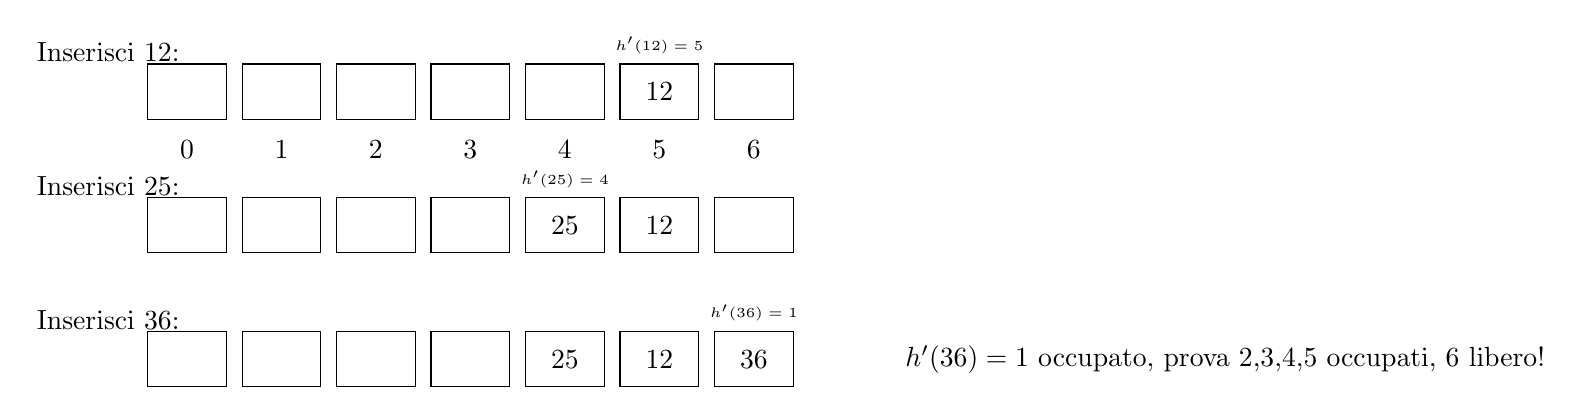
\begin{tikzpicture}[
    box/.style={rectangle, draw, minimum width=1cm, minimum height=0.7cm}
]
% Passo 1
\node at (-1, 2.5) {Inserisci 12:};
\foreach \i in {0,...,6} {
    \node[box] (a\i) at (\i*1.2, 2) {};
    \node[below] at (\i*1.2, 1.5) {\i};
}
\node at (a5) {12};
\node[above] at (a5.north) {\tiny $h'(12)=5$};

% Passo 2
\node at (-1, 0.8) {Inserisci 25:};
\foreach \i in {0,...,6} {
    \node[box] (b\i) at (\i*1.2, 0.3) {};
}
\node at (b5) {12};
\node at (b4) {25};
\node[above] at (b4.north) {\tiny $h'(25)=4$};

% Passo 3
\node at (-1, -0.9) {Inserisci 36:};
\foreach \i in {0,...,6} {
    \node[box] (c\i) at (\i*1.2, -1.4) {};
}
\node at (c5) {12};
\node at (c4) {25};
\node at (c6) {36};
\node[above] at (c6.north) {\tiny $h'(36)=1$};
\node[right] at (9, -1.4) {$h'(36)=1$ occupato, prova 2,3,4,5 occupati, 6 libero!};
\end{tikzpicture}
\end{center}

\textbf{Problema:} \textit{Primary clustering} -- si formano lunghe sequenze contigue di celle occupate, peggiorando le prestazioni.

\subsubsection{Quadratic Probing}

\begin{definizione}[Quadratic probing]
\[
h(k, i) = (h'(k) + c_1 i + c_2 i^2) \bmod m
\]
dove $c_1, c_2$ sono costanti.
\end{definizione}

Esempio comune: $c_1 = c_2 = 1$, quindi $h(k, i) = (h'(k) + i + i^2) \bmod m$.

\textbf{Vantaggio:} Riduce il primary clustering.

\textbf{Problema:} \textit{Secondary clustering} -- chiavi con lo stesso hash iniziale seguono la stessa sequenza di probe.

\subsubsection{Double Hashing}

\begin{definizione}[Double hashing]
\[
h(k, i) = (h_1(k) + i \cdot h_2(k)) \bmod m
\]
dove $h_1, h_2$ sono funzioni hash ausiliarie.
\end{definizione}

\textbf{Requisiti:}
\begin{itemize}
    \item $h_2(k)$ deve essere relativamente primo con $m$ (se $m$ è primo, basta $h_2(k) \neq 0$)
    \item Comune: $m = 2^p$ e $h_2(k)$ dispari, oppure $m$ primo
\end{itemize}

\textbf{Esempio:}
\begin{align*}
h_1(k) &= k \bmod m \\
h_2(k) &= 1 + (k \bmod (m-1))
\end{align*}

\textbf{Vantaggio:} Minimizza clustering, approssima hashing uniforme.

\textbf{Operazioni con open addressing:}

\begin{lstlisting}[style=pseudocode]
def insert(T, k, v):
    """
    Inserimento con open addressing
    Complessità: O(1/(1-α)) in media
    """
    i = 0
    while i < m:
        j = h(k, i)
        if T[j] == None or T[j] == DELETED:
            T[j] = (k, v)
            return j
        i = i + 1

    errore "Tabella piena"

def search(T, k):
    """
    Ricerca con open addressing
    """
    i = 0
    while i < m:
        j = h(k, i)
        if T[j] == None:
            return None  // chiave non presente
        if T[j].key == k:
            return T[j].value
        i = i + 1

    return None
\end{lstlisting}

\textbf{Cancellazione:} Non possiamo semplicemente mettere \texttt{None}, altrimenti spezziamo le catene di probe. Soluzione: marcare la cella come \texttt{DELETED} (tombstone).

\begin{teorema}[Complessità con open addressing]
Con hashing uniforme, il numero atteso di probe è:
\begin{itemize}
    \item Ricerca senza successo: $\frac{1}{1-\alpha}$
    \item Ricerca con successo: $\frac{1}{\alpha} \ln \frac{1}{1-\alpha}$
\end{itemize}
dove $\alpha = n/m < 1$ è il fattore di carico.
\end{teorema}

\textbf{Osservazione:} Con $\alpha = 0.5$ (tabella metà piena), ricerca senza successo richiede in media 2 probe. Con $\alpha = 0.9$, servono 10 probe!

\textbf{Pratica:} Mantenere $\alpha < 0.7$ per buone prestazioni.

\section{Confronto delle tecniche}

\begin{center}
\begin{tabular}{|l|c|c|}
\hline
\textbf{Caratteristica} & \textbf{Chaining} & \textbf{Open Addressing} \\
\hline
Memoria extra & Puntatori & No \\
$\alpha$ può superare 1 & Sì & No \\
Cancellazione & Semplice & Complessa (tombstones) \\
Località cache & Scarsa & Buona \\
Prestazioni con $\alpha$ alto & Degrada linearmente & Degrada rapidamente \\
Implementazione & Più semplice & Più complessa \\
\hline
\textbf{Migliore per} & $\alpha$ variabile & $\alpha$ basso, memoria limitata \\
\hline
\end{tabular}
\end{center}

\section{Analisi formale}

\begin{definizione}[Hashing uniforme semplice]
Assumiamo che ogni chiave abbia uguale probabilità $1/m$ di finire in ogni slot, indipendentemente da dove finiscono le altre chiavi.
\end{definizione}

\begin{teorema}[Lunghezza attesa delle liste nel chaining]
Sotto hashing uniforme semplice, la lunghezza attesa di una lista è $\alpha = n/m$.
\end{teorema}

\begin{proof}
Sia $X_i$ il numero di elementi nella lista $i$. Per linearità del valore atteso:
\[
E[X_i] = E\left[\sum_{j=1}^{n} \mathbb{1}[\text{chiave } j \text{ va in slot } i]\right] = \sum_{j=1}^{n} P[\text{chiave } j \text{ in slot } i] = \sum_{j=1}^{n} \frac{1}{m} = \frac{n}{m} = \alpha
\]
\end{proof}

\begin{teorema}[Costo di ricerca con successo nel chaining]
Il costo atteso di una ricerca con successo è $1 + \alpha/2$.
\end{teorema}

\begin{proof}[Idea]
In media, dobbiamo scansionare metà della lista contenente la chiave cercata. La lunghezza media è $\alpha$, quindi $1 + \alpha/2$ (il $+1$ per calcolare l'hash).
\end{proof}

\section{Applicazioni pratiche}

Le tabelle hash sono onnipresenti:

\begin{itemize}
    \item \textbf{Database}: Indici hash per accesso rapido
    \item \textbf{Compilatori}: Tabelle dei simboli
    \item \textbf{Caching}: Memorizzazione di risultati precedenti
    \item \textbf{Set e dizionari}: Python \texttt{dict}, Java \texttt{HashMap}, C++ \texttt{unordered\_map}
    \item \textbf{Deduplicazione}: Rilevare elementi duplicati in $O(n)$
    \item \textbf{Crittografia}: Hash crittografici (SHA-256, MD5 -- non per tabelle hash!)
    \item \textbf{Blockchain}: Hash dei blocchi
    \item \textbf{Password storage}: Hash di password (con salt)
\end{itemize}

\section{Hash crittografici vs hash per tabelle}

\textbf{Differenze fondamentali:}

\begin{center}
\begin{tabular}{|l|p{5cm}|p{5cm}|}
\hline
& \textbf{Hash per tabelle} & \textbf{Hash crittografici} \\
\hline
\textbf{Scopo} & Distribuzione uniforme & Sicurezza \\
\hline
\textbf{Velocità} & Più veloce possibile & Può essere lento \\
\hline
\textbf{Collisioni} & Accettabili, gestite & Devono essere computazionalmente intrattabili \\
\hline
\textbf{Reversibilità} & Irrilevante & Deve essere one-way \\
\hline
\textbf{Dimensione output} & Piccola ($\log m$ bit) & Grande (256+ bit) \\
\hline
\textbf{Esempi} & $k \bmod m$, MurmurHash & SHA-256, SHA-3, BLAKE2 \\
\hline
\end{tabular}
\end{center}

\textbf{Attenzione:} NON usare hash crittografici per tabelle hash (troppo lenti), e NON usare hash per tabelle in contesti di sicurezza!

\section{Tabelle hash perfette}

\begin{definizione}[Perfect hashing]
Un \textbf{perfect hash} è una funzione hash senza collisioni per un insieme statico di chiavi.
\end{definizione}

Se l'insieme di chiavi è noto a priori e non cambia, possiamo costruire una tabella hash perfetta che garantisce $O(1)$ nel \textbf{caso peggiore} (non solo in media).

\textbf{Schema a due livelli:}
\begin{enumerate}
    \item Prima funzione hash $h: U \to \{0, \ldots, m-1\}$
    \item In ogni slot $i$, seconda tabella hash con $m_i = n_i^2$ slot (dove $n_i$ è il numero di chiavi in slot $i$)
\end{enumerate}

\begin{teorema}[Perfect hashing]
Con hashing universale a due livelli, si può costruire una tabella hash perfetta con spazio $O(n)$ e tempo di ricerca $O(1)$ worst-case.
\end{teorema}

\textbf{Applicazioni:} Compilatori, riserve di parole chiave, dizionari statici.

\section{Bloom Filters}

Un'applicazione avanzata dell'hashing sono i \textbf{Bloom filters}, strutture dati probabilistiche per test di appartenenza.

\textbf{Proprietà:}
\begin{itemize}
    \item Spazio: $O(n)$ bit (molto compatto)
    \item Inserimento: $O(k)$ dove $k$ è il numero di funzioni hash
    \item Ricerca: $O(k)$
    \item \textbf{Falsi positivi possibili, falsi negativi NO}
\end{itemize}

\textbf{Applicazioni:} Database distribuiti, web caching, bioinformatica.

\section{Esercizi}

\subsection{Esercizio 1}
Progettare una funzione hash per numeri di telefono italiani (10 cifre).

\subsection{Esercizio 2}
Dimostrare che con chaining e $\alpha = 1$, il numero atteso di probe per ricerca senza successo è 1.

\subsection{Esercizio 3}
Implementare una tabella hash con double hashing.

\subsection{Esercizio 4}
Calcolare il numero atteso di collisioni quando si inseriscono $n$ chiavi in una tabella di dimensione $m$.

\subsection{Esercizio 5}
Progettare una tabella hash che supporta \texttt{deleteRandom()} in $O(1)$ ammortizzato.

\section{Conclusioni}

Le tabelle hash sono strutture dati fondamentali che offrono prestazioni eccezionali:

\textbf{Punti chiave:}
\begin{itemize}
    \item Operazioni in tempo medio $O(1)$ -- inarrivabile per BST
    \item Funzione hash cruciale: deve distribuire uniformemente
    \item Collisioni inevitabili: gestirle con chaining o open addressing
    \item Fattore di carico $\alpha$ determina prestazioni
    \item Chaining: semplice, robusto a $\alpha$ alto
    \item Open addressing: compatto, buona località cache
    \item Rehashing dinamico per mantenere $\alpha$ basso
    \item Perfect hashing per insiemi statici: $O(1)$ worst-case
\end{itemize}

\textbf{Quando usare hash table:}
\begin{itemize}
    \item Serve accesso rapido per chiave
    \item Non serve ordinamento
    \item Non serve ricerca per range
    \item Spazio non è critico
\end{itemize}

\textbf{Quando usare BST/AVL:}
\begin{itemize}
    \item Serve ordinamento
    \item Serve ricerca per range
    \item Serve navigazione ordinata (min, max, successore)
\end{itemize}

Le tabelle hash, insieme ad array, liste, alberi e grafi, formano il toolkit essenziale delle strutture dati. La scelta appropriata tra queste strutture, basata sulle operazioni richieste e sui vincoli di prestazioni, è una competenza fondamentale per ogni informatico.

\textbf{Prospettive future:}

Esistono molte varianti avanzate di tabelle hash: cuckoo hashing, hopscotch hashing, Robin Hood hashing, ognuna con diversi trade-off tra prestazioni, semplicità e garanzie worst-case. L'esplorazione di queste varianti è un'area di ricerca attiva, particolarmente importante per sistemi concorrenti e distribuiti.

\vspace{1cm}

\begin{center}
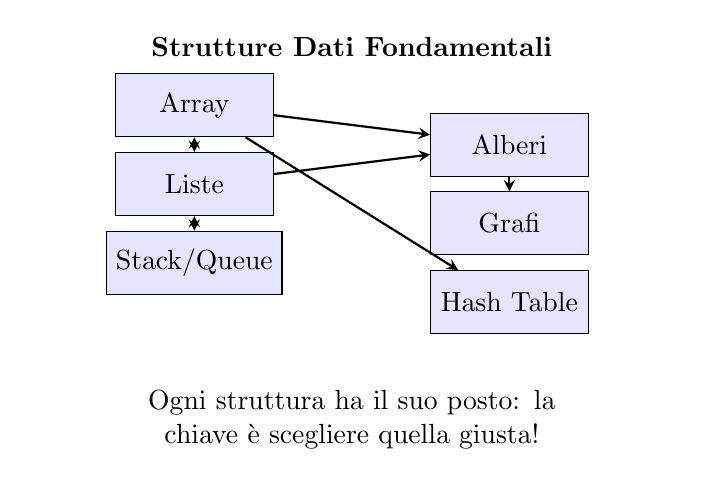
\begin{tikzpicture}[
    box/.style={rectangle, draw, minimum width=2cm, minimum height=0.8cm, fill=blue!10},
    >=stealth
]
\node[box] (array) at (0,3) {Array};
\node[box] (list) at (0,2) {Liste};
\node[box] (stack) at (0,1) {Stack/Queue};
\node[box] (tree) at (4,2.5) {Alberi};
\node[box] (graph) at (4,1.5) {Grafi};
\node[box] (hash) at (4,0.5) {Hash Table};

\node[above] at (2, 3.5) {\textbf{Strutture Dati Fondamentali}};

\draw[<->, thick] (array) -- (list);
\draw[<->, thick] (list) -- (stack);
\draw[->, thick] (array) -- (tree);
\draw[->, thick] (list) -- (tree);
\draw[->, thick] (tree) -- (graph);
\draw[->, thick] (array) -- (hash);

\node[below, text width=8cm, align=center] at (2, -0.5) {
    Ogni struttura ha il suo posto: la chiave è scegliere quella giusta!
};
\end{tikzpicture}
\end{center}

\textit{Fine del capitolo sulle tabelle hash.}
